% Paper draft: feature-space ambiguity investigation (F2S3 + GeDi, TCH landslide)
% Build:  pdflatex main && pdflatex main
% Figures: python make_figures.py   (regenerates figures/ from investigate/out/)
\documentclass[11pt,a4paper]{article}

\usepackage[margin=2.5cm]{geometry}
\usepackage{amsmath,amssymb}
\usepackage{graphicx}
\usepackage{booktabs}
\usepackage{xcolor}
\usepackage[font=small,labelfont=bf]{caption}
\usepackage[colorlinks=true,linkcolor=blue!50!black,citecolor=blue!50!black,urlcolor=blue!50!black]{hyperref}
\usepackage{lineno}
\linenumbers

\graphicspath{{figures/}}

% ---- draft machinery: highlight what is still missing ------------------------
\newcommand{\missing}[1]{%
  \par\noindent\fcolorbox{orange!80!black}{orange!8}{\parbox{0.965\linewidth}{%
    \small\textbf{\textcolor{orange!80!black}{Missing for submission:}} #1}}\par\medskip}
\newcommand{\missinginline}[1]{\textcolor{orange!80!black}{[\textbf{missing:} #1]}}

% ---- notation ----------------------------------------------------------------
\newcommand{\Ns}{N_s}
\newcommand{\Nt}{N_t}
\newcommand{\vv}{\lvert v\rvert}

\title{Feature-space ambiguity, not descriptor collapse, causes residual
  gross outliers in deep-feature point-cloud displacement estimation:\\
  a diagnostic study on a rocky landslide}
\author{\missinginline{author list and affiliations}\\[2pt]
  \small Draft v0.1 --- code in \texttt{investigate/}, branch
  \texttt{feature\_descriptor\_gedi}}
\date{}

\begin{document}
\maketitle

\begin{abstract}
\noindent
Learned local descriptors have made dense 3D displacement estimation between
terrestrial laser-scanning (TLS) epochs practical, but on natural,
self-similar terrain the resulting vector fields can contain spatially
clustered gross outliers that survive downstream geometric filtering. Using
the F2S3 pipeline with GeDi descriptors on two epochs of a rocky landslide
with moraine-like structures, we diagnose the mechanism behind these
outliers. We show that (i)~the descriptors do not degenerate --- among
861{,}552 source descriptors, none has a near-duplicate --- yet (ii)~the raw
nearest-neighbour correspondence field is 67\% gross outliers, because for a
median source point \emph{four} target candidates are within 10\% of the best
match's feature distance, and these near-tied candidates are scattered across
the entire tile (median spatial spread 277\,m on a 479\,m tile). The
ambiguity is therefore deeper than the second neighbour: a top-2 Lowe ratio
test is structurally blind to it for the 69\% of points with more than two
near-tied candidates, and a depth-10 ratio $r_{10}=d_1/d_{10}$ predicts
surviving outliers markedly better ($\mathrm{AUC}=0.797$) than the Lowe ratio
($0.636$). An offline filter simulation reveals a complementary,
practice-relevant result: the best \emph{thresholded} filter is not the best
AUC metric --- a spatial-spread test with poor AUC (0.607) reduces the raw
outlier rate from 67\% to 2.4\% and, composed with the pipeline's supervoxel
filter, yields a 0.47\% outlier skeleton, six times cleaner than the
strictest ratio test at comparable retention. All conclusions are invariant
to the outlier-label threshold over 20--60\,m. The study motivates
ambiguity-aware rejection in the matching stage and, longer term,
descriptors optimised for distinctiveness on self-similar natural surfaces.
\end{abstract}

\missing{The abstract quantifies results from a single tile of a single
scene. Before submission it must either be re-scoped as a case study or be
backed by the planned multi-tile / full-resolution replication
(Sec.~\ref{sec:limitations}).}

\section{Introduction}\label{sec:intro}

Geodetic deformation monitoring increasingly relies on dense 3D displacement
vector fields estimated directly between point clouds of two epochs. F2S3
\cite{gojcic2020} pioneered a feature-based formulation: a deep local
descriptor is computed for every point, each source point is assigned its
nearest neighbour in \emph{feature space} as corresponding target point, and
implausible correspondences are rejected by enforcing local rigid-body
consistency inside supervoxels. Unlike surface-differencing methods (C2C,
M3C2), this recovers the full 3D displacement vector, including motion
tangential to the surface.

The correspondence step, however, contains no notion of \emph{match
reliability}: every source point receives a partner, however weak the
evidence. On the rocky landslide studied here (Sec.~\ref{sec:data}), the
filtered displacement field is largely coherent (median
$\vv\approx7.6$\,m over $\sim$11 months), but $4.6\%$ of the plotted vectors
are gross outliers of tens to hundreds of metres. They are not isolated
noise: they form spatially clustered blobs in visually low-texture regions
(uniform debris and moraine-like surfaces), which suggests a systematic
matching failure rather than random noise, and they survive the supervoxel
filter that should remove them.

Two classical remedies --- Lowe's ratio test \cite{lowe2004} and a
mutual-nearest-neighbour check --- examine only the best one or two matches.
Before adopting either, we test a sharper hypothesis:

\begin{quote}
\textbf{H:} On self-similar terrain the descriptor is not sufficiently
distinctive: for many source points the \emph{entire} top-$k$ feature
neighbourhood --- not just the second neighbour --- is near-tied, and the
near-tied candidates are scattered across the tile. This ambiguity is the
mechanism behind the surviving outlier blobs, and a top-2 ratio test can
capture it only partially.
\end{quote}

From H we derive five questions: (Q1)~are the descriptors themselves
degenerate, i.e.\ do many points share near-identical descriptors within one
epoch? (Q2)~how sharply does the best cross-epoch match stand out from its
runners-up? (Q3)~where do the near-tied candidates sit \emph{in space}?
(Q4)~which ambiguity measure best predicts the observed outliers? (Q5)~which
rejection rule achieves the best density/purity trade-off? Each question
maps to one experiment (Sec.~\ref{sec:results}); a sensitivity analysis
verifies that the answers do not depend on the outlier-labelling threshold.

\paragraph{Contributions.}
(1)~A diagnosis separating two failure modes that are often conflated ---
descriptor \emph{collapse} (many identical descriptors) versus descriptor
\emph{indistinctiveness} (distinct descriptors that cannot rank the true
partner first) --- with evidence that only the latter occurs here.
(2)~Quantitative evidence that matching ambiguity on natural terrain is
\emph{deep} (median four-way near-ties) and \emph{spatially global} (median
candidate spread 277\,m), which explains why top-2 tests underperform.
(3)~A methodological caution: filter selection by AUC alone would have
discarded the best-performing filter; operating-point (Pareto) analysis is
required. (4)~A validated, reproducible evaluation protocol for
correspondence ambiguity in deep-feature displacement pipelines, including
a proxy-label defence and an approximate-search validity check.

\section{Related work}\label{sec:related}

\missing{This section has not been researched yet. It should cover, at
minimum: (i)~point-cloud deformation monitoring baselines (C2C, M3C2,
supervoxel-based and piecewise-ICP methods); (ii)~learned local 3D
descriptors (3DMatch, FCGF, DIP, GeDi, and successors) and their reported
distinctiveness properties; (iii)~match-reliability tests in 2D and 3D
feature matching (ratio test, mutual NN, second-nearest-in-other-cluster,
learned match filters such as context normalisation / attention-based
filtering); (iv)~repetitive-structure ambiguity in place recognition and
SLAM (perceptual aliasing), which is the closest analogue to the phenomenon
studied here. Currently the bibliography holds only the four works cited
directly.}

\section{Pipeline, data, and labels}\label{sec:data}

\subsection{The F2S3 pipeline in brief}

F2S3 \cite{gojcic2020} processes an epoch pair in four stages:
(1)~voxel-grid downsampling and tiling; (2)~per-point deep local feature
descriptors --- here GeDi \cite{poiesi2022}, a rotation-invariant descriptor
producing $D=32$ dimensions in our configuration; (3)~correspondence search:
each source descriptor is assigned its (approximate) nearest target
descriptor using HNSW \cite{malkov2018}; the displacement vector of a source
point is the offset to its matched target point; (4)~outlier filtering: the
source cloud is segmented into supervoxels, a rigid motion is robustly
estimated per supervoxel, and correspondences inconsistent with it are
discarded. Only stage-(4) survivors are written to the output displacement
field.

\subsection{Scene and run configuration}

The test scene (``TCH'') is a rocky landslide with moraine-like structures,
observed by TLS at two epochs, 2021-09-24 and 2022-08-31 ($\sim$11 months
apart). We analyse the spatially subsampled working clouds used during
parameter tuning, processed as a single tile with $\Ns=861{,}552$ source and
$\Nt=775{,}358$ target points at 0.2\,m voxel size, descriptor neighbourhood
radius 6\,m, supervoxel radius 4\,m. This configuration reproduces the
production outlier pattern and is the setting in which the outlier blobs
were first observed.

\missing{Scene metadata required for a paper and not derivable from the
repository: instrument and scanning geometry, point density of the raw
clouds, co-registration procedure and its accuracy between the epochs, and
geographic/geological description of the landslide. These must be provided
by the operators.}

\subsection{Two displacement fields, and a data-integrity correction}
\label{sec:fields}

Two fields must be distinguished throughout:

\begin{itemize}
  \item \textbf{Raw 1-NN field} --- the matcher's own output before any
  filtering: one vector per source point. This is the field the descriptor
  is directly responsible for.
  \item \textbf{Survivor field} --- the subset kept by the supervoxel
  filter; this is what the pipeline writes out and what the operator plots.
\end{itemize}

A correction discovered during validation: the output file is \emph{not}
row-aligned with the feature matrices --- the pipeline writes only surviving
points, reordered by supervoxel (189{,}034 rows against 861{,}552 source
points). Any analysis joining per-point metrics to the output by row index
would silently compare unrelated points. We therefore recompute all
magnitudes from the correspondence archive (row-aligned by construction) and
recover the survivor set by exact 6-D coordinate matching of output rows
into correspondence rows, verified to zero magnitude error on all rows.

\begin{table}[t]
\centering
\caption{The two displacement fields of the analysed tile. The supervoxel
filter turns a two-thirds-outlier raw field into the plotted field; the
4.63\% residual outliers are the clustered blobs that motivated this study.}
\label{tab:fields}
\begin{tabular}{lrrr}
\toprule
field & points & median $\vv$ & share $\vv\ge40$\,m\\
\midrule
raw 1-NN        & 861{,}552 \ (100\%) & 96.1\,m & \textbf{67.2\%}\\
survivors       & 189{,}034 \ (21.9\%) & 7.61\,m & 4.63\%\\
\bottomrule
\end{tabular}
\end{table}

Table~\ref{tab:fields} contains the first substantive finding: \textbf{the
raw matching output is two-thirds gross outliers}. The supervoxel filter is
not polishing an essentially correct field --- it is rescuing a broken one,
and the residual blobs are its leakage.

\subsection{Outlier labels: a defended proxy, not ground truth}
\label{sec:labels}

No independent reference exists for this scene --- no GNSS, no manually
verified correspondences, no identified stable areas. All ``outlier'' labels
in this study are therefore a \emph{proxy}: a correspondence is labelled a
gross outlier when $\vv\ge\theta$, with $\theta=40$\,m as working value. Two
observations defend the proxy (Fig.~\ref{fig:magnitude}):

\begin{enumerate}
  \item \textbf{Bimodality.} The survivor magnitude distribution has a
  coherent-motion mode ($93.3\%$ below 15\,m) and a scattered far tail
  ($3.3\%$ beyond 100\,m); only $0.66\%$ of survivors fall anywhere between
  25\,m and 60\,m. Any threshold inside that valley labels nearly the same
  point set.
  \item \textbf{Threshold invariance.} Every ranking reported below was
  recomputed at five thresholds $\theta$ between 20 and 60\,m
  (Sec.~\ref{sec:sensitivity}); no ordering of metrics or filters changes.
\end{enumerate}

What the proxy cannot do is validate individual vectors: a wrong match that
lands by chance at a plausible displacement is invisible to it, so all
purity numbers are \emph{lower bounds} on the true error rate.

We use four recurring point groups: \emph{raw outliers}
($\vv\ge40$\,m, any point; 578{,}677 = 67.2\% of $\Ns$); \emph{survivors}
(kept by the supervoxel filter; 189{,}034); \emph{trusted} points (survived
and $\vv<15$\,m; 176{,}435); and \emph{residual outliers} (survived and
$\vv\ge40$\,m; 8{,}756 = 4.63\% of survivors --- the blobs). The
\emph{baseline} operating point of the current pipeline is the survivor
field: 21.9\% density at 4.63\% outliers.

\begin{figure}[t]
\centering
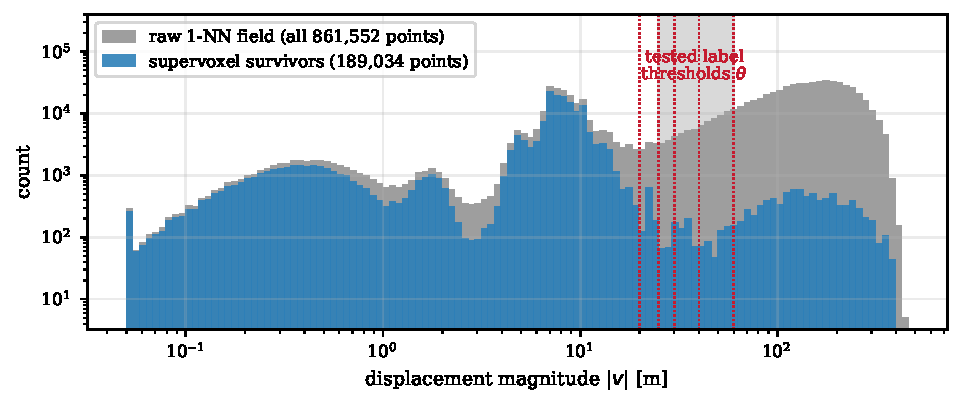
\includegraphics[width=\linewidth]{fig_magnitude.pdf}
\caption{Displacement-magnitude distributions (log--log). The survivor
field (blue) is strongly bimodal: coherent motion below $\sim$15\,m and a
far outlier tail, separated by a sparsely populated valley (shaded,
25--60\,m) in which all tested label thresholds $\theta$ (dotted) lie. The
raw 1-NN field (grey) is dominated by a broad gross-outlier hump at
$\vv>40$\,m.}
\label{fig:magnitude}
\end{figure}

\subsection{Validity of exact \texorpdfstring{$k$}{k}-NN analysis for the
HNSW-based pipeline}\label{sec:hnsw}

All analyses use exact (brute-force, GPU-chunked) $k$-nearest-neighbour
search, while the pipeline uses approximate HNSW. If the two disagreed
materially, our metrics would describe a different matcher than the one that
produced the field. On this tile the HNSW-chosen partner equals the exact
1-NN for $99.960\%$ of source points (343 disagreements out of 861{,}552);
in every disagreement the HNSW pick lies within the exact top-20, with a
median feature-distance excess of 1.5\% (95th percentile 8.6\%). Exact-kNN
statements therefore transfer to the production matcher.

\section{Ambiguity metrics}\label{sec:metrics}

For source point $i$, let $d_1\le d_2\le\dots\le d_{20}$ denote its sorted
L2 distances to the 20 nearest target descriptors (computed once and reused
by all experiments).

\paragraph{Lowe ratio.} $r_2=d_1/d_2$ \cite{lowe2004}. Values near 1 mean
the runner-up is nearly as good as the winner; the classical criterion
accepts a match if $r_2<0.8$. It sees exactly one competitor.

\paragraph{Deep ratio.} $r_{10}=d_1/d_{10}$, and the equivalent
$\mathrm{flatness}=(d_{10}-d_1)/d_1=1/r_{10}-1$. These are ad-hoc
extensions defined for this study (no literature source claimed); being
monotone transforms of each other they are identical under rank-based
evaluation and we report only $r_{10}$.

\paragraph{Ambiguity depth.}
$\mathrm{depth}_\varepsilon=\#\{\,j\le20 : d_j\le(1+\varepsilon)\,d_1\,\}$
for $\varepsilon\in\{0.05,0.1,0.2\}$. Here $\varepsilon$ is a
\emph{relative distance tolerance}: $\mathrm{depth}_{0.1}$ counts the
candidates within 10\% of the winner's distance --- how many are
``effectively tied for first place''. Depth 1 means the winner stands
alone; depth $\gg2$ is precisely the regime a top-2 test cannot represent.
There is no canonical $\varepsilon$, so we report three and let the
predictive evaluation and the sensitivity analysis judge.

\paragraph{Spatial spread.} Map the top-10 candidates to their coordinates
and take the maximum pairwise Euclidean distance among them. Spread is the
only \emph{geometric} measure: it asks not how close the runner-up
\emph{distances} are, but where the alternative matches would put the
point.

\paragraph{Within-epoch self-similarity (collapse test).}
$d^{\mathit{self}}_1(i)$ is the distance from source descriptor $i$ to its
nearest \emph{other} source descriptor, and $n_\varepsilon(i)$ counts other
source descriptors within an absolute radius
$\varepsilon_1=0.1\cdot\mathrm{median}(d^{\mathit{self}}_1)$. Unlike the
depth tolerance, $\varepsilon_1$ is a single global radius tied to the data
scale (one tenth of the typical nearest-neighbour distance), so
$n_\varepsilon$ counts \emph{near-duplicates} rather than merely close
descriptors.

\paragraph{Evaluation score.} We score each metric's ability to separate
outliers from non-outliers by the area under the ROC curve (AUC) ---
equivalently, the probability that a randomly drawn outlier has a larger
metric value than a randomly drawn non-outlier --- computed rank-based with
tie correction; 0.5 means no information, 1.0 perfect separation. The AUC is unrelated to the
$\varepsilon$ parameters: $\varepsilon$ shapes a metric's values, AUC then
scores those values against the labels of Sec.~\ref{sec:labels}.

\missing{No uncertainty quantification yet: AUC values and outlier rates
are point estimates. Bootstrap confidence intervals (resampling source
points, or better, spatial block bootstrap to respect spatial correlation)
should be added.}

\section{Results}\label{sec:results}

Each subsection states the expectation under hypothesis H before the
observation, and flags deviations.

\subsection{Q1: No descriptor collapse}\label{sec:collapse}

\emph{Expectation under H:} if GeDi degenerates on self-similar surfaces,
large regions should show $d^{\mathit{self}}_1\approx0$ and
$n_\varepsilon\gg0$.

\emph{Observation (Fig.~\ref{fig:t1}):} the opposite. Median
$d^{\mathit{self}}_1=0.211$, giving $\varepsilon_1=0.021$; $n_\varepsilon=0$
for \emph{every one} of the 861{,}552 source descriptors --- not a single
descriptor has even one near-duplicate within its own epoch. GeDi does not
collapse on this terrain.

This negative result sharpens H rather than refuting it: the failure mode is
not ``the network emits the same vector everywhere'' but ``the vectors,
while distinct, do not place the correct partner first by a reliable
margin'' (Secs.~\ref{sec:profile}--\ref{sec:depth}). It also predicts,
correctly, that $n_\varepsilon$ carries no information about outliers
(AUC exactly 0.500, Table~\ref{tab:auc}).

\begin{figure}[t]
\centering
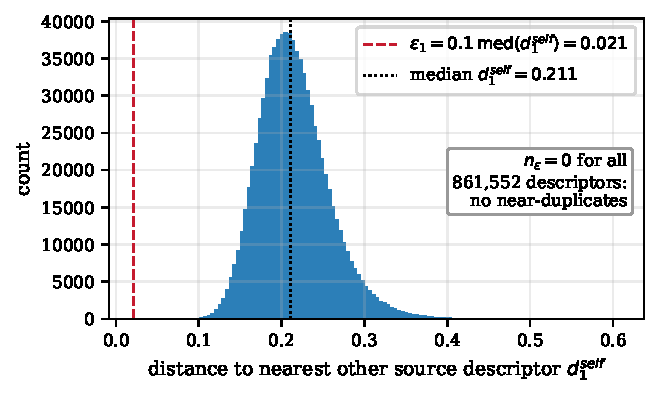
\includegraphics[width=0.6\linewidth]{fig_t1_selfsim.pdf}
\caption{Within-epoch self-similarity of the source descriptors. The
distance to the nearest other descriptor is bounded far away from the
near-duplicate radius $\varepsilon_1$ (dashed): no descriptor collapse.}
\label{fig:t1}
\end{figure}

\subsection{Q2a: The winner barely stands out}\label{sec:profile}

\emph{Expectation under H:} trusted points should show a distance profile
that rises steeply after $d_1$ (a distinct winner), residual outliers a flat
profile. In an ideal world the $(d_1,r_2)$ distribution would concentrate at
$r_2\ll1$ --- a clear winner for every point.

\emph{Observation (Fig.~\ref{fig:t2}):} ambiguity manifests as mass piling
up against $r_2\to1$ for the bulk of all points. Group means: $r_2=0.919$
(trusted) versus $0.951$ (residual outliers); $r_{10}=0.766$ versus
$0.858$. Two consequences. First, even for \emph{trusted} points the
runner-up is on average only $\sim$8\% worse than the winner --- far from
the ideal-world picture --- so classical Lowe filtering at $r_2<0.8$ would
discard the overwhelming majority of correct matches on this terrain (it
keeps 1.4\% of all points, Table~\ref{tab:pareto}). Second, the group
separation in $r_2$ (0.032) is one third of the separation in $r_{10}$
(0.092): first evidence that the discriminative signal lives deeper than
rank 2.

\begin{figure}[t]
\centering
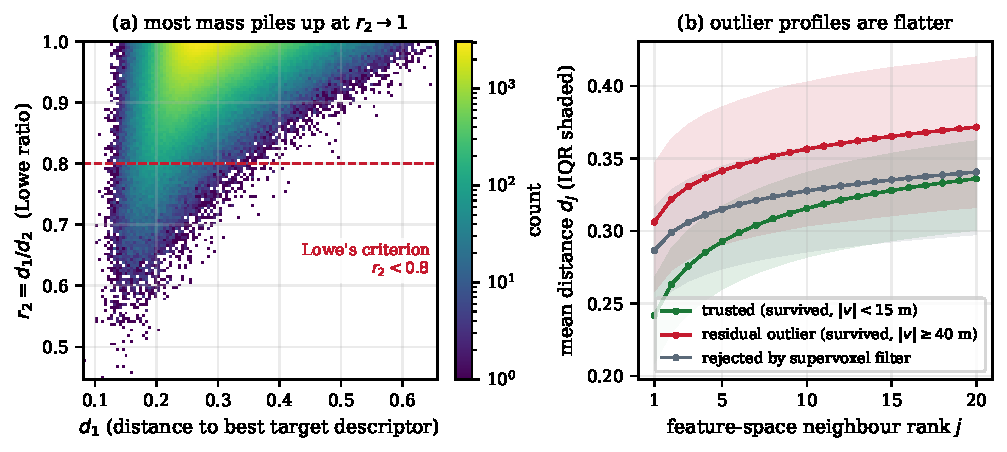
\includegraphics[width=\linewidth]{fig_t2_profile.pdf}
\caption{Cross-epoch match quality. (a)~Joint density of best-match
distance $d_1$ and Lowe ratio $r_2$ (log colour scale): most points sit
near $r_2\to1$, i.e.\ the runner-up is nearly as good as the winner;
Lowe's classical acceptance region lies below the dashed line. (b)~Mean
top-20 distance profiles by group (bands: interquartile range): residual
outliers (red) have flatter profiles than trusted points (green), but the
difference is gradual, not categorical.}
\label{fig:t2}
\end{figure}

\subsection{Q2b: The ambiguity is deep}\label{sec:depth}

\emph{Expectation under H:} residual outliers should have
$\mathrm{depth}\gg2$ far more often than trusted points, and a substantial
fraction of all points at depth $>2$ would prove a top-2 test structurally
blind here.

\emph{Observation (Fig.~\ref{fig:t3}):} confirmed. At $\varepsilon=0.1$ the
median ambiguity depth is \textbf{4}, and \textbf{69.3\%} of all source
points have depth $>2$; group means are 2.92 (trusted) versus 5.81
(residual outliers). For over two thirds of the points, the situation a
top-2 ratio test models --- one winner, one challenger --- simply does not
exist; there is a cluster of challengers.

\emph{Caveat:} at $\varepsilon=0.2$ the median depth equals $20=k$, i.e.\
the statistic is right-censored by the top-20 search; true depths at loose
tolerance are larger than reported ($k=100$ would be needed to measure
them). This does not affect any ranking below, which uses $\varepsilon=0.1$.

\begin{figure}[t]
\centering
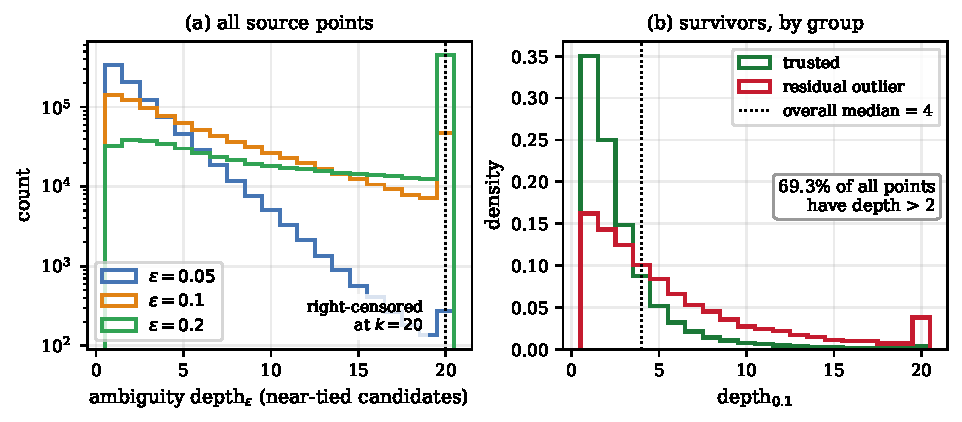
\includegraphics[width=\linewidth]{fig_t3_depth.pdf}
\caption{Ambiguity depth. (a)~Depth distributions for three tolerance
values (log counts); the spike at 20 is censoring by the top-$k$ search,
not data. (b)~At $\varepsilon=0.1$, residual outliers (red) are shifted to
systematically larger depths than trusted points (green); the overall
median is 4.}
\label{fig:t3}
\end{figure}

\subsection{Q3: Near-tied candidates are scattered across the tile}
\label{sec:spread}

\emph{Expectation under H:} trusted points $\to$ small spread (candidates
cluster around the true partner); ambiguous points $\to$ spread approaching
the tile diameter.

\emph{Observation (Fig.~\ref{fig:t4}):} the second half is confirmed
emphatically --- median spread of the top-10 candidates is \textbf{277\,m on
a tile with a 479\,m diagonal} (90th percentile 343\,m). The alternative
matches of a typical point are not local jitter around the true partner;
they are distributed over the entire scene, which is exactly the mechanism
that converts a near-tie in feature space into a hundreds-of-metres blunder
in the displacement field.

\emph{Deviation from expectation:} trusted points \emph{also} show large
mean spread (220\,m versus 262\,m for residual outliers). Global candidate
scatter is near-universal on this terrain; what distinguishes reliable
points is membership in the small-spread \emph{tail} (spread
$<10$--$20$\,m), not a low average. This asymmetry explains the seemingly
paradoxical behaviour of spread in
Secs.~\ref{sec:predict}--\ref{sec:pareto}.

\begin{figure}[t]
\centering
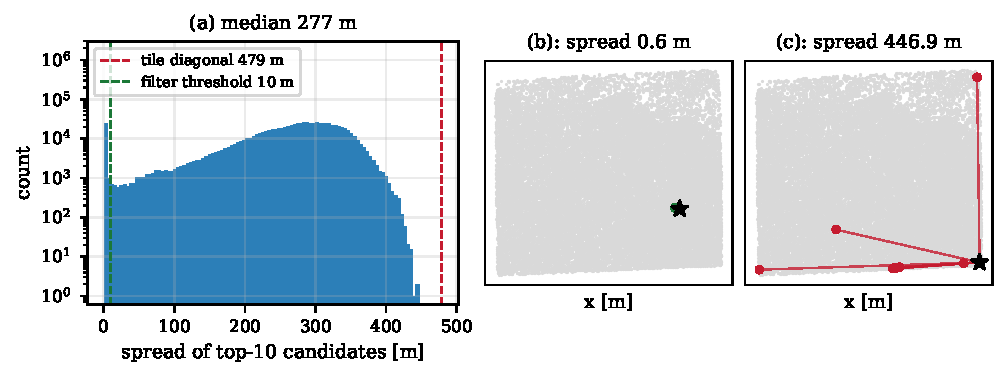
\includegraphics[width=\linewidth]{fig_t4_spread.pdf}
\caption{Spatial spread of the top-10 candidate sets. (a)~Distribution
(log counts): the mass sits at hundreds of metres, with a distinct
low-spread spike near zero. (b)~A distinctive point: all 10 candidates
coincide at the source location (green dots hidden behind the star).
(c)~An ambiguous point: near-tied candidates span the full tile. Grey:
target cloud (subsampled), top view.}
\label{fig:t4}
\end{figure}

\subsection{Q4: Which metric predicts the outliers?}\label{sec:predict}

\emph{Expectation under H:} depth- and spread-type metrics should outrank
the top-2 ratio in AUC.

\emph{Observation (Table~\ref{tab:auc}, Fig.~\ref{fig:t5}):} confirmed for
the depth direction: $r_{10}$ (AUC 0.797 on the residual target) decisively
outranks $r_2$ (0.636) --- the discriminative information sits between ranks
2 and 10, invisible to a top-2 test. Two unexpected results: (i)~the raw
match distance $d_1$ alone is nearly as predictive as $r_{10}$ among
survivors (0.791): a large absolute feature distance is itself a strong
warning sign; (ii)~spread scores second-worst (0.607) --- yet
Sec.~\ref{sec:pareto} shows it is the best \emph{filter}, a contradiction
resolved there.

\begin{table}[t]
\centering
\caption{AUC of each ambiguity metric as a predictor of the gross-outlier
label ($\vv\ge40$\,m), for the raw target (all source points) and the
residual target (supervoxel survivors only). Flatness is omitted: it is a
monotone transform of $r_{10}$ with identical AUC.}
\label{tab:auc}
\begin{tabular}{lcc}
\toprule
metric & raw target & residual target\\
\midrule
$r_{10}=d_1/d_{10}$        & 0.781 & \textbf{0.797}\\
$d_1$ (match distance)      & 0.680 & 0.791\\
depth$_{0.2}$               & 0.765 & 0.772\\
depth$_{0.1}$               & 0.712 & 0.699\\
depth$_{0.05}$              & 0.641 & 0.629\\
$r_2$ (Lowe ratio)          & 0.640 & 0.636\\
spread (top-10)             & 0.629 & 0.607\\
$n_\varepsilon$ (collapse)  & 0.500 & 0.500\\
\bottomrule
\end{tabular}
\end{table}

\begin{figure}[t]
\centering
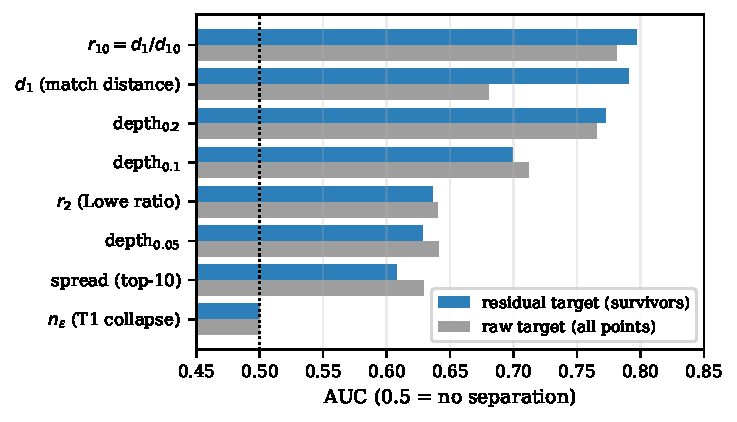
\includegraphics[width=0.62\linewidth]{fig_t5_auc.pdf}
\caption{Separability (AUC) of the ambiguity metrics for both targets,
sorted by the residual target. The collapse count $n_\varepsilon$ is
exactly uninformative, consistent with Sec.~\ref{sec:collapse}.}
\label{fig:t5}
\end{figure}

\subsection{Q5: Filter operating points and the Pareto view}
\label{sec:pareto}

Every candidate rejection rule is a boolean mask over source points, so its
effect can be simulated offline. Because a feature-space filter would run
\emph{before} the (unchanged) supervoxel filter, each rule is evaluated as
the intersection of both filters and quoted as an \emph{operating point}:
retained density (\% of all $\Ns$; baseline 21.9\%) versus outlier rate
among kept points. Rule A \emph{dominates} rule B if it is simultaneously
denser and cleaner; the set of non-dominated rules is the \emph{Pareto
frontier} --- the menu of rational choices --- and the ``knee'' is where
sacrificing more density stops buying meaningful purity.

\emph{Expectation under H:} a depth- or spread-based rejection should reach
a better operating point than the ratio test.

\emph{Observation (Table~\ref{tab:pareto}, Fig.~\ref{fig:t6}):}

\begin{enumerate}
  \item \textbf{Like-for-like, depth beats ratio.} At matched density
  (12.8\% vs 12.5\%), $\mathrm{depth}_{0.1}\le2$ yields 2.42\% outliers
  versus 3.10\% for $r_2<0.95$. The AUC conclusion carries through to
  operating points.
  \item \textbf{Spread is the best single filter by a wide margin, despite
  its poor AUC.} Acting alone on the raw field it cuts 67.2\% $\to$ 2.4\%
  outliers while keeping 3.0\% of points; composed with the supervoxel
  filter it reaches 2.1\% density at \textbf{0.47\%} outliers ---
  $\sim$6$\times$ cleaner than the strictest ratio test at comparable
  retention. Resolution of the AUC contradiction: AUC scores a metric's
  ranking over its \emph{entire} range, but spread is uninformative over
  most of its range (Sec.~\ref{sec:spread}: nearly everything scatters
  widely) and nearly pure in its low tail. A low-recall/high-precision
  signal loses at AUC and wins as a thresholded filter.
  \emph{Methodological consequence: selecting a filter by AUC alone would
  have picked $r_{10}$ and discarded the strongest filter.}
  \item \textbf{Mutual NN alone is insufficient} (50.2\% outliers on the
  raw field): when the descriptor cannot rank the true partner first, the
  wrong assignment is often symmetric, so the mutuality check passes.
  \item The median $\vv$ is stable (7.3--7.8\,m) under every rule: the
  central motion estimate was never in question; the rules differ only in
  how much of the tail they admit.
  \item No rule dominates the baseline: every gain in purity costs
  density. The choice of knee depends on downstream use
  (Sec.~\ref{sec:conclusion}).
\end{enumerate}

\begin{table}[t]
\centering
\caption{Filter operating points (selection; full grid in
\texttt{investigate/out/t6\_pareto\_tile\_000.csv}). ``Kept'' is the
density after composing the rule with the supervoxel filter; ``raw alone''
is the outlier rate of the rule applied to the raw 1-NN field without the
supervoxel filter.}
\label{tab:pareto}
\small
\begin{tabular}{lcccc}
\toprule
filter & kept [\% of $\Ns$] & outliers [\%] & median $\vv$ [m] & raw alone [\%]\\
\midrule
none (baseline)                       & 21.9 & 4.63 & 7.61 & 67.2\\
depth$_{0.1}\le3$                     & 16.0 & 2.73 & 7.61 & 49.8\\
depth$_{0.1}\le2$                     & 12.8 & 2.42 & 7.62 & 46.3\\
$r_2<0.95$                            & 12.5 & 3.10 & 7.62 & 54.8\\
mutual NN                             &  8.6 & 1.54 & 7.49 & 50.2\\
$r_2<0.80$ (Lowe's value)             &  1.4 & 0.67 & 7.78 & 14.6\\
spread $<10$\,m                       &  2.1 & \textbf{0.47} & 7.32 & \textbf{2.4}\\
mutual $\wedge$ $r_2<0.9$ $\wedge$ spread$<10$\,m & 0.5 & 0.13 & 7.31 & 0.6\\
\bottomrule
\end{tabular}
\end{table}

\begin{figure}[t]
\centering
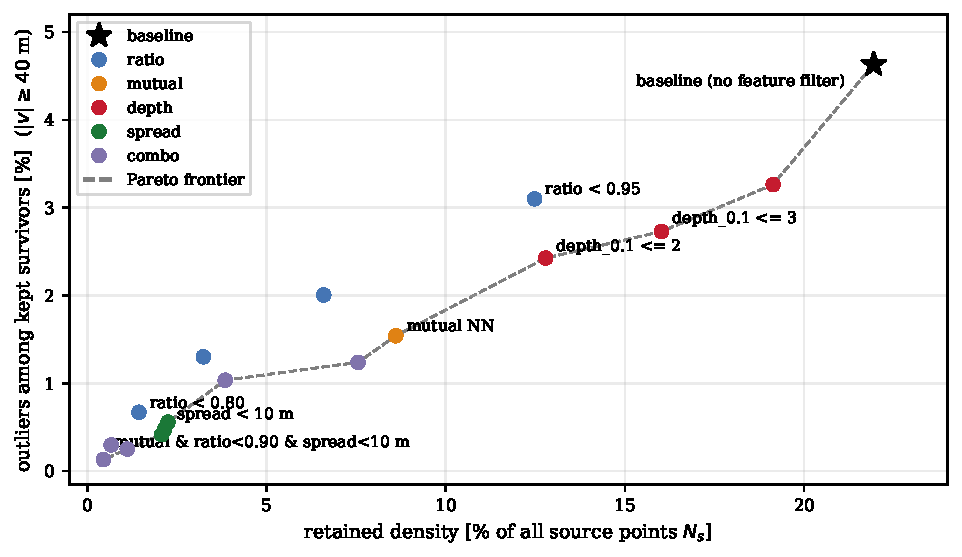
\includegraphics[width=0.85\linewidth]{fig_t6_pareto.pdf}
\caption{Density--purity operating points of all simulated rejection rules
(composed with the supervoxel filter). The dashed line is the Pareto
frontier. The spread family (green) occupies the low-density, very-low
outlier corner; the depth family (red) traces the frontier at high
density.}
\label{fig:t6}
\end{figure}

\subsection{Robustness to the label threshold}\label{sec:sensitivity}

Recomputing base rates, all metric AUCs, and all filter outlier rates at
$\theta\in\{20,25,30,40,60\}$\,m changes no ordering anywhere in the range
(Fig.~\ref{fig:t7}; e.g.\ spread $<10$\,m moves from 0.76\% to 0.43\%
outliers monotonically). Combined with the bimodality of
Fig.~\ref{fig:magnitude}, the proxy label is as solid as it can be made
without reference data.

\begin{figure}[t]
\centering
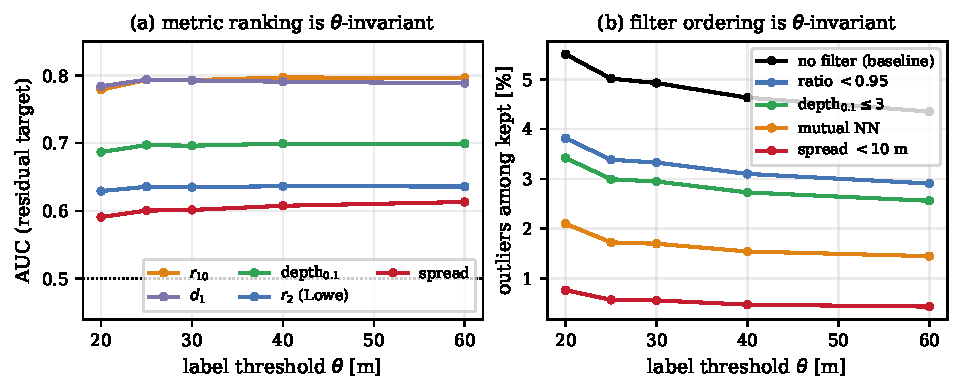
\includegraphics[width=\linewidth]{fig_t7_sensitivity.pdf}
\caption{Sensitivity to the outlier-label threshold $\theta$: (a)~metric
AUCs and (b)~filter outlier rates vary smoothly and never change order for
$\theta\in[20,60]$\,m.}
\label{fig:t7}
\end{figure}

\section{Discussion}\label{sec:discussion}

\paragraph{The hypothesis, revisited.} H is confirmed in its mechanism,
refuted in one detail, and exceeded in one respect. \emph{Confirmed:} the
surviving outlier blobs arise from feature-space ambiguity that is deeper
than the second neighbour (median four-way near-ties; 69\% of points beyond
the reach of a top-2 test; $r_{10}\gg r_2$ in predictive power), and the
near-tied candidates scatter across the full tile, which converts ambiguity
into large blunders. \emph{Refuted detail:} there is no descriptor collapse;
the descriptors are distinct but insufficiently separated to rank reliably.
\emph{Exceeded:} the raw 1-NN field is 67\% gross outliers --- the problem
is not a blemish on a good matching stage; the supervoxel filter currently
carries the pipeline.

\paragraph{No filter adds information.} Because the descriptors are
individually distinct (Sec.~\ref{sec:collapse}) yet collectively ambiguous,
rejection tests can only \emph{remove} unreliable points, never recover
correct partners the descriptor failed to rank first. Every operating point
in Fig.~\ref{fig:t6} trades density for purity; none dominates the
baseline. Genuine improvement requires either additional evidence at
matching time (spatial regularisation, geometric verification of candidate
sets --- the spread result shows the geometry of the candidate set carries
information the feature distances do not) or a more distinctive descriptor
on this terrain class.

\paragraph{AUC is not filter quality.} The spread metric ranks second-worst
by AUC yet provides the cleanest practical filter. Threshold-free
separability scores reward metrics that rank well \emph{everywhere};
deployment only needs a metric that is trustworthy \emph{somewhere} (here:
the low-spread tail). Filter selection should therefore always include an
operating-point analysis; in this study, an AUC-only protocol would have
selected $r_{10}$ and discarded the best filter.

\section{Limitations}\label{sec:limitations}

\begin{enumerate}
  \item \textbf{Proxy labels.} All purity numbers rest on $\vv\ge\theta$;
  wrong matches with plausible magnitudes are uncounted, so purity values
  are lower bounds. Mitigated by bimodality and threshold invariance;
  removable only with reference data.
  \item \textbf{Single tile, scene, and configuration.} All numbers
  describe one tile of the TCH sample clouds with GeDi-32 at 6\,m radius.
  Generalisation to full-resolution clouds, other scenes, other
  descriptors (e.g.\ DIP-64), and other radii is untested.
  \item \textbf{Censoring.} depth$_{0.2}$ is right-censored at $k=20$.
  \item \textbf{Unoptimised thresholds.} The filter grid is coarse; the
  true frontier may lie between grid points.
  \item \textbf{Runtime cost unmeasured.} The spread filter needs a
  top-10 search and mutual NN a reverse search; the wall-clock cost of
  upgrading the correspondence stage from $k=1$ has not been measured.
\end{enumerate}

\missing{Items to resolve before submission, in priority order:
(1)~replication on further tiles and the full-resolution epoch pair;
(2)~a reference dataset --- identified stable (bedrock) areas or manually
verified correspondences --- to replace the proxy label for at least a
subset of points; (3)~bootstrap confidence intervals for
Tables~\ref{tab:auc} and \ref{tab:pareto}; (4)~a $k{=}100$ re-run to
de-censor depth$_{0.2}$; (5)~runtime measurements for the $k\ge10$
correspondence stage; (6)~the DIP-64 descriptor as a comparison
condition.}

\section{Conclusions and future work}\label{sec:conclusion}

On a rocky landslide with self-similar debris surfaces, the residual gross
outliers of a deep-feature displacement pipeline are caused by deep,
spatially global matching ambiguity --- not by degenerate descriptors. The
practical consequences are immediate: (i)~a rejection filter belongs in the
correspondence stage, exposed as an opt-in option; for a downstream user
who densifies the field (e.g.\ RBF interpolation), the spread $<10$\,m rule
offers an extremely clean skeleton (0.47\% outliers), while
$\mathrm{depth}_{0.1}\le3$ preserves 73\% of current density with 41\%
fewer outliers if the field is used as-is; (ii)~evaluation protocols for
such filters must report operating points, not only AUC. Future work:
exploiting the spatial coherence of candidate sets at matching time, and
training or fine-tuning descriptors for distinctiveness on self-similar
natural terrain, which is where the information bottleneck demonstrably
lies.

\missing{Author contributions, acknowledgements, funding, and data/code
availability statements.}

\begin{thebibliography}{9}\small

\bibitem{gojcic2020}
Z.~Gojcic, C.~Zhou, A.~Wieser.
\newblock F2S3: Robustified determination of 3D displacement vector fields
using deep learning.
\newblock \emph{Journal of Applied Geodesy}, 14(2), 2020.

\bibitem{poiesi2022}
F.~Poiesi, D.~Boscaini.
\newblock Learning general and distinctive 3D local deep descriptors for
point cloud registration.
\newblock \emph{IEEE Transactions on Pattern Analysis and Machine
Intelligence}, 45(3), 2022.

\bibitem{malkov2018}
Y.~A. Malkov, D.~A. Yashunin.
\newblock Efficient and robust approximate nearest neighbor search using
hierarchical navigable small world graphs.
\newblock \emph{IEEE Transactions on Pattern Analysis and Machine
Intelligence}, 42(4), 2018.

\bibitem{lowe2004}
D.~G. Lowe.
\newblock Distinctive image features from scale-invariant keypoints.
\newblock \emph{International Journal of Computer Vision}, 60(2), 2004.

\end{thebibliography}

\missing{Bibliography is limited to the four directly used sources; the
related-work survey (Sec.~\ref{sec:related}) will add the remainder.
Reference details (volume/issue/pages) should be verified --- they were
filled from memory, not from the publishers' records.}

\end{document}
